\documentclass[11pt, english]{article}

\title{{\bf Travelling Salesman Problem (TSP)}}
\author{Louise Harding \\ Robin Khatri \\ Laetitia Couge\\ Mohammed Paul Doust \\ Mohammed Nassar}

\date{\today}


\usepackage[T1]{fontenc}
\usepackage{babel}
\usepackage{geometry}
\usepackage{titling}
\usepackage{hyperref}
\usepackage{graphicx}	
\usepackage{float,flafter}
\renewcommand\maketitlehooka{\null\mbox{}\vfill}
\renewcommand\maketitlehookd{\vfill\null}
\usepackage{blindtext}
\usepackage[utf8]{inputenc}	
%\usepackage{algorithm}	
\usepackage{algorithmic}	
\usepackage[absolute,overlay]{textpos}
\usepackage{graphicx}
\setlength{\droptitle}{-4em}     % Eliminate the default vertical space
\addtolength{\droptitle}{-4pt}   % Only a guess. Use this for adjustment
\usepackage[export]{adjustbox}
\usepackage{amsmath}
\usepackage{caption}	
\usepackage{subcaption}	
\usepackage{subfiles}
\usepackage{amsmath,amssymb,amsfonts,textcomp}
\usepackage{inputenc}
\usepackage{algorithm2e}
\usepackage{xcolor}
\usepackage[flushleft]{threeparttable}
\begin{document}
\newcommand\tab[1][1.2cm]{\hspace*{#1}}

\begin{titlingpage}
\maketitle
\center 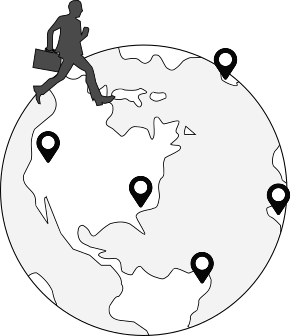
\includegraphics[scale=0.5]{tsp.png}

\end{titlingpage}
\tableofcontents
\newpage

\section{Introduction}

Consider a salesman who has to visit a set of cities and return to the city he started from, provided he visits each city only once.\\
\\
\noindent
The problem is to minimize the total cost or distance of the route. This is known as the Travelling Salesman Problem.\\
\\
\noindent
The problem can be summarised as follows: \\
\\
\tab TSP = $\{(G,f,t)$: $G = (V,E)$ is a complete graph,\\
\tab \tab $f$ is a function $V\times V \rightarrow Z,$\\
\tab \tab $t \in Z,$ \\
\tab \tab $G$ is a graph that contains a travelling salesman tour with costs or distances that\\ \tab \tab does not exceed $t\}$.

\subsection{Symmetric Travelling Salesman Problem}

If in a travelling salesman problem, cost or distance of travelling from city $i$ to city $j$ is equal to the cost or distance of travelling from city $j$, $i.e.$ the cost matrix is symmetric, then the problem is said to be \emph{Symmetric Travelling Salesman Problem}.

\subsection{Asymmetric Travelling Salesman Problem}

If in a travelling salesman problem, cost or distance of travelling from city $i$ to city $j$ can differ from the cost or distance of travelling from city $j$, $i.e.$ the cost matrix is asymmetric, then the problem is said to be \emph{Asymmetric Travelling Salesman Problem}. A real world example could be routes consisting of some one-way roads.


\subsection{Sparsity of TSP}


A graph with only a few edges is referred to as a sparse graph. In our testing with different exact and approximate algorithms, we have tested on problems of varying sparsity levels.

\newpage
\section{Brute Force Algorithm}
\subsection{Introduction}
Bruteforce algorithm runs through all possible solutions and selects the best one. It is not an optimal algorithm to use for TSP with a large number of nodes.

\subsection{Experiment and complexity}

We tested the code on both symmetric and asymmetric problems. Since it provides exacts solutions, the solutions were optimal.\\

\noindent
The complexity of the algorithm is $\mathcal{O}(n!)$. We tested it on tsp's up to 10 cities, as the complexity increased rapidly after that.

\begin{center}
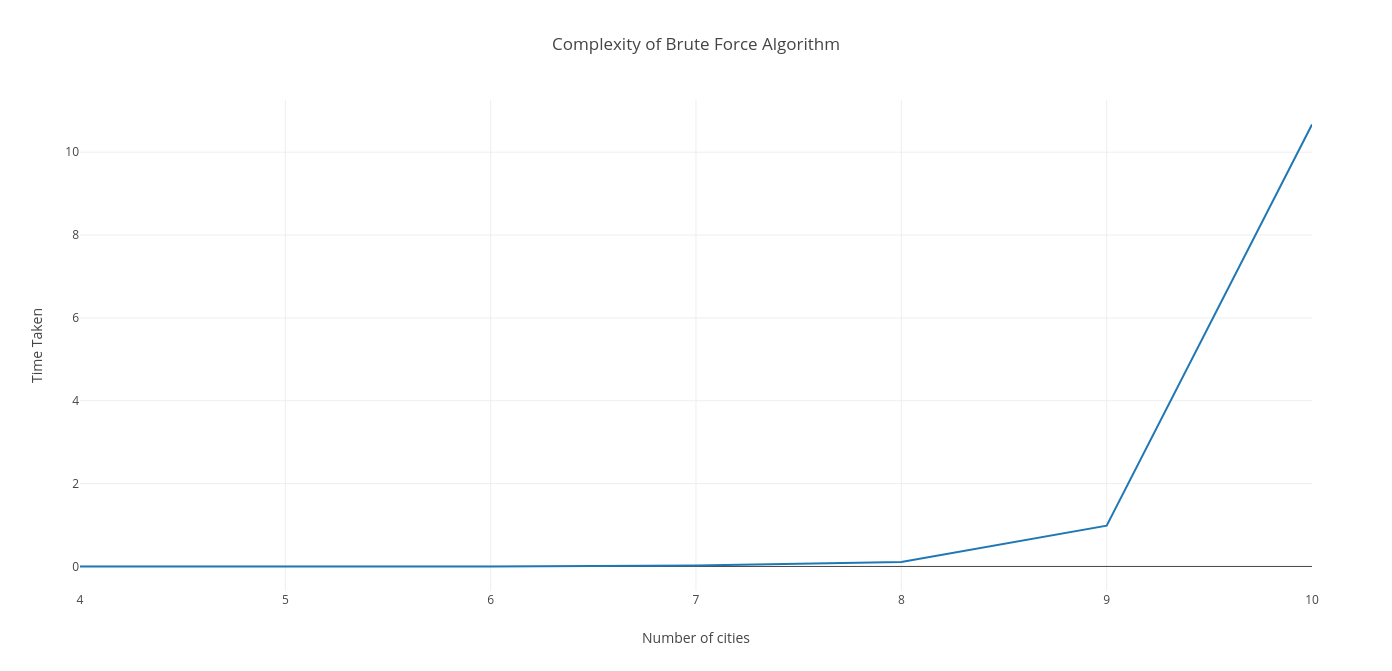
\includegraphics[scale=0.3]{bruteforce.png}
\end{center}

\noindent
In case of Symmetric TSPs, the computational time can be reduced by computing distances only for permutations which begin with our choice of first city. However, the complexity still remains $\mathcal{O}(n!)$, but number of permutations to cover decrease.\\
\\
\noindent
Improvements on Bruteforce Algorithm are provided with Branch and Bound Algorithms presented in the next section.


\newpage
\section{Branch and Bound - Matrix Reduction method}
\subsection{Introduction}
A branch-and-bound algorithm consists of a systematically looking for the shortest path by searching a state space tree : the approach tries to minimise the initial depth first search by selecting the lest cost path option at each decision point (node) in the tree. Once this first cost (upper bound) is found the cost at each node is evalated in future searches of the tree and if it exceeds the value, the tree is pruned and the lower branches are not searched.

\subsection{Approach}
The approach used for this algorithm was the one presented in class. Starting with an adjecency matrix, subtract the minimum edge weight for all values in the same row and then do the same for the columns, the sum of the values subtracted equals the lower bound for this tsp problem. After the initial matrix reduction, using a state space tree, map the possible edges from the starting node (root) and choose the one with the least weight. With this node, using the vertex it corresponds to, set the represented row values in the matrix to infinity, and the matrix values that represents the reverse of this edge (eg if going for 1 to 2, we set 2 to 1) to infinity. Repeat this process until the first leaf is reached. This provides the first upper bound. 
Continue this process by backtracking up and down the tree, each time checking for the upper bound. If the upper bound is smaller, update the upper bound. If it is larger, then prune the branch.

\subsection{Complexity}
\noindent
The complexity of this algorithm is at worst $\mathcal{O}(n!)$, which is the same as Brute Force, because this happens in the case where no pruning of the braches occurs. In practice, however, it will be better than this as the entire space will not need to be searched.

\subsection{Testing}
Due to the complexity Brand and Bound takes too long to run against the TSP library, so we tested it against a variety of generated tsp problems. We tested the code on both symmetric and asymmetric problems, with differing levels of sparcity. As expected the number of vertices dramatically increased the time, up until about 13 vertices fully connected to each other taking greater than 1 hour. \newline 
The sparcity of the connections between vertices affected the time taken due to less connections results in a smaller search area. There were mixed results with symmetric vs asymetric with neither showing to be consistently easier to process than the other, most likely the pruning between the different problems resulted in less clear results. We also tested it against Brute force and it did in reality produce faster results.

\begin{figure}[H]
\centering
\begin{subfigure}{.33\textwidth}
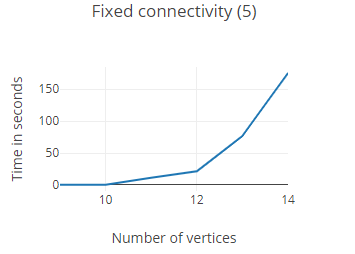
\includegraphics[height=5cm,valign=t]{fixed_connectivity.png}
\caption{Example of increase in vertex count}
\end{subfigure}%
\hfill
\begin{subfigure}{.33\textwidth}
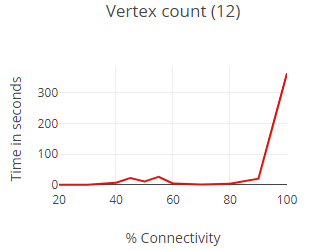
\includegraphics[height=5cm,valign=t]{fixed_vertices.png}
\caption{Example of increase in connectivity}
\end{subfigure}%
\end{figure}

\section{Branch and Bound with Adding and Removing Edges}
\subsection{Introduction}
One of the strategies used for searching the solution space is Branch and Bound which keeps dividing the space into branches. one for solutions containing a given edge and the other for those excluding the given edge. forming a binary tree as follows:
\newline \newline
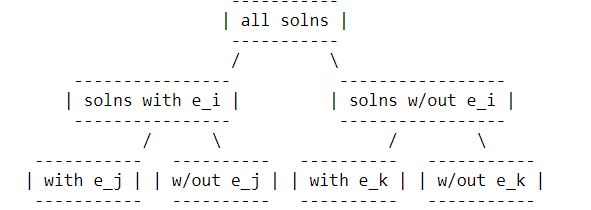
\includegraphics[width=\textwidth] {solution-tree.jpg}
\newline \newline
The main parts of these algorithm are:
\begin{enumerate}
    \item Bounding Function
    \item Choosing Splitting Edge
    \item How to Include Edge
    \item How to Exclude Edge
\end{enumerate}

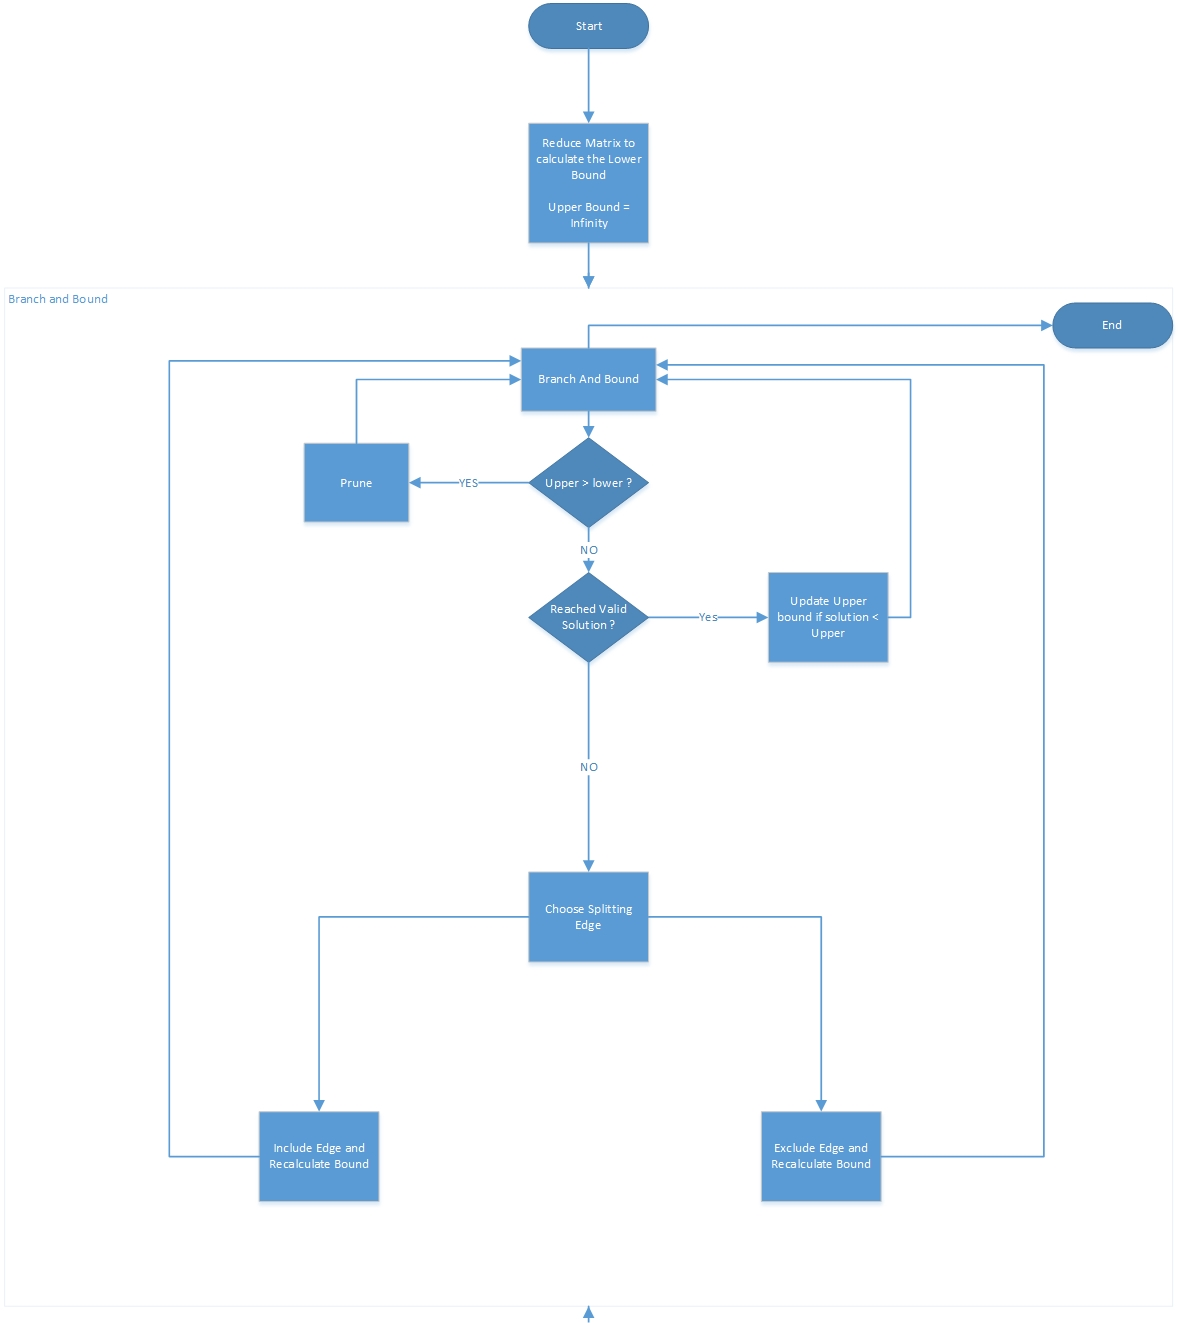
\includegraphics[width = \textwidth]{bnb-flow.jpg}

\subsection{Bounding Function (Reduction)}
The solution is bounded by normalizing the solution matrix. this is done by reducing the rows first and the columns after.
by reducing the Rows/Columns we mean normalizing them. we subtract the minimum element from each row from each element at that row. and the same for columns. at the end we will have a matrix with at least one zero in each column and each row.
Our lower bound will be the sum of all minimum values with used to reduce the matrix.

\subsection{Choosing Splitting Edge}
We are looking to maximize the right part by trying to raising the lower bound of the right sub-tree. In order to do that, we choose to split on the edge that best maximize the lower bound. We look for the zero weight edges that maximize the increasing in the lower bound.

\subsection{How to Include Edge}
Including an edge (ie, I -> J) is done by first, forbidding the going back from J -> I by setting the weight of edge J -> to INFINITY ( we also forbid the going back to any sub-path in our partial solution). Moreover, since we have used this edge, we cannot go from node i to any other node, and similarly, we cannot reach node J. Consequently, we delete the I th row and the J th column from our solutions matrix.
in the end, we reduce the new matrix after including the edge.

\subsection{How to Exclude Edge}
To exclude edge (ie, I-> J), we start by setting the cost of the edge I->J to INFINITY. and we reduce the new matrix afterwards.

\subsection{Complexity}

\begin{center}
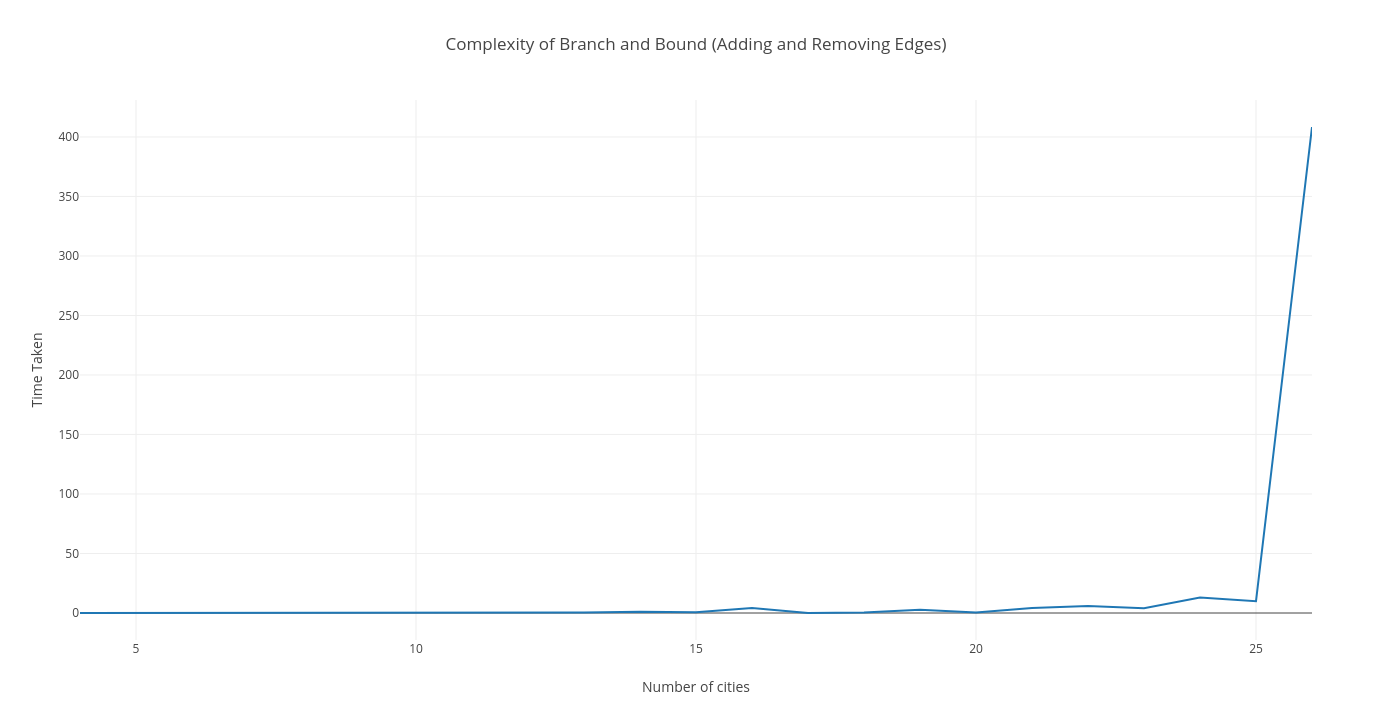
\includegraphics[scale=0.22]{branchandbound.png}
\end{center}

\section{Randomized algorithm}	
\subfile{algo_random}	
 \section{Dynamic Programming algorithm}	
\subfile{algo_dp}	

\section{Ant Colony Algorithm}

\subsection{Introduction}

Ant Colony Algorithm is a probabilistic algorithm that takes inspiration from the behavior of ants to Travelling Salesman Problems. The first algorithm that took inspiration from ants was described in 1992 by Marco Dorigo in his PhD thesis \cite{Dorigothesis}. Later, there has been various optimization techniques building upon this research. In 2004, book titled Ant Colony Optimzation was published. We took inspiration from this book for our implementation of Ant Colony Algorithm.

\subsection{Behavior of Ants}

\begin{center}
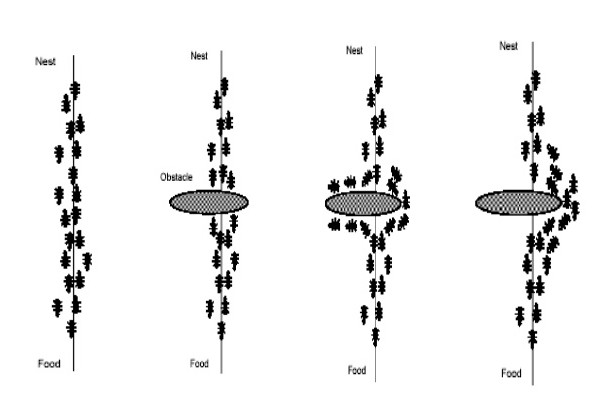
\includegraphics[scale=0.5]{antfood.jpg}
\end{center}

Ants live together in colonies and they form a highly structured societies. Ants do not have a developed visual skills and some of the species of ants are blind. They, however, make use of pheromones which they leave behind while naviagting. This is a form of indirect communication with other ants in the colony. Due to high concentration of pheromones on a path, ants are influenced to take the path previously travelled by the former ants. This behavior leads to the convergence of establishing a path, \emph{i.e.} after a certain time, all the ants which are travelling together follow the same path (and find the food!)
 
\subsection{Theory}

The behavior of ants described above can be utilised to form an algorithm able to provide approximate solutions to TSP problems.\\

\noindent
Consider $m$ ants and they are placed in $n$ cities chosen randomly from the list of cities in our problem.\\
\\
\begin{center}
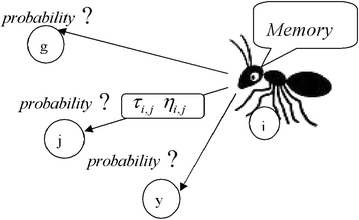
\includegraphics[scale=0.5]{ant.png}
\end{center}

\noindent
Ant number $k$ moves from city $i$ to city $j$ with probability $p_{ij}^m$ given below:

\begin{center}
$p_{ij}^k = \frac{{(\tau_{ij}^\alpha)(\eta_{ij}^\beta)}}{\sum_{ij \rightarrow allowed}{(\tau_{ij}^\alpha)(\theta_{ij}^\beta)}}$
\end{center}
\noindent
Where, $\tau_{ij}$ is the amount of pheromone deposited for transition from city \emph{i} to \emph{j}.

\tab  $\eta _{ij}$ is the desirability of going to city ${j}$ from city ${i}$. It is given by ${1/d_{ij}}$.

\tab $\alpha$ and $\beta$ are parameters that respectively control the influence of $\tau_{ij}$ and $\eta _{xy}$.\\

\noindent
Many special cases of Ant Colony Optimzation has been proposed. In this project, we have considered Ant Colony System (ACS) \cite{Dorigo1997}. Other popular approaches are Ant System (Earliest Ant Colony Algorithm)\cite{Dorigo06antcolony} and MAX-MIN Ant System (MMAS)\cite{Sttzle1998}. These Optimization methods differ in their approach of updating pheromones and calculating transition probabilities $p_{ij}$. \\
\\
\noindent
{\bf Ant System (AS)}:\\
\\
In AS,\\
\noindent
Updates of pheromones:\\ 
When all ants complete their tours, trails of pheromones are updated as follows:

\begin{center}
$\tau_{ij} = (1-\rho).\tau_{ij} + \sum_{k}\Delta \tau_{ij}^k$
\end{center}
where $\Delta \tau_{ij}^k$ can be calculated depending upon the strategy we choose, and $\rho$ is the evaporation rate. Higher the $\rho$, quicker is the evaporation rate of pheromones.\\
\begin{center}
$\Delta \tau _{ij}^{k}={\begin{cases}Q/L_{k}&{\mbox{if ant }}k{\mbox{ uses transition city }}i \rightarrow j{\mbox{ in its tour}}\\0&{\mbox{otherwise}}\end{cases}}$\\
\end{center}
\noindent
Where $L_{k}$ is the cost of ant k's tour, and Q is a constant.\\

\noindent
{\bf Ant Colony System (ACS)}: \\
\\
In ACS,\\
The local pheromone update is done by each ant k after every transition $i \rightarrow j$. Each ant applies this update to the last edge it transversed.
\begin{center} {$\tau_{ij} = (1-\phi).\tau_{ij} + \phi.\tau_{0}$} \end{center}
Where $\tau_{0}$ is the initial value of the phreromone (Usually kept small) and $\phi$ is the pheromone decay coefficient. After a complete travel, the local updates are deleted.\cite{Dorigo1997}\\

\noindent
Secondly, after all ants have completed the paths, the global update of pheromone is done only taking into account the best tour so far. In this case, 

\begin{center}
$\tau_{ij} = (1-\rho).\tau_{ij} + \Delta \tau_{ij}^{best}$
\end{center}
\noindent
Where,
\begin{center}
$\Delta \tau _{ij}^{best}={\begin{cases}Q/L_{Best}&{\mbox{if best ant}}{\mbox{ uses transition city }}i \rightarrow j{\mbox{ in its tour}}\\0&{\mbox{otherwise}}\end{cases}}$\\
\end{center}
\noindent
$L_{Best}$ is the total length of the best path so far, and Q is a constant.\\
 
\subsection{Algorithm}

\begin{enumerate}
	\item Initialize parameters
	\item Randomly place m ants in n cities
	\item Choose transitions
	\begin{enumerate}
		\item Calculate $p_{ij}$ using equation given above. 
		\item trasit from city {i} to {j} randomly based on probabilities $p_{ij}$ and locally update pheromones
	\end{enumerate}	 
	\item When all ants have completed a solution, choose best solution and globally update pheromones using aforementioned expressions and remove local updates
	\item Iterate the process
\end{enumerate}

\subsection{Results on TSPLIB Problems}
We chose $\alpha$ to be 1 and $\beta$ to be 10. We have not experimented with other values of these parameters, however, there is literature suggesting choice of these hueristics but solutions were close to optimal. Choice of number of ants depend on the number of cities in our problem. In general we considered number of ants to be close to the number of cities. \\ 
\\
In our experiments, number of ants were chosen to be in a range of [10,50], and number of iterations we chose to were in a range of (100-200).\\
\\
Since TSPLIB contains repository of TSPs which vary in their sparsity and range of elements in cost matrix, therefore as a benchmark of the algorithm, we tested the algorithm on TSPLIB problems. For this purpose, we considered both Symmetric and Assymetric TSP Problems from TSPLIB database, and solutions are presented below:

\begin{table}[h!]
  \begin{center}
    \caption{Observed vs Optimal solutions}
    \label{tab:table1}
    \begin{tabular}{c|c|c|c|c|c}
      \textbf{Dataset} & \textbf{No. of cities} & \textbf{No. of ants} & \textbf{Iterations} & \textbf{Solution found}  &\textbf{Opt. solution}\\ % 
      \hline
      {burma14.tsp} & 14 & 10 & 100 & 3381 & 3323 \\ % <--
      {ulysses16.tsp} & 16 & 10 & 100 & 6987 & 6859 \\ 
	 {att48.tsp} & 48 & 40 & 200 & 10725 & 11153 \\ % <--
	 {berlin52.tsp} & 52 & 40 & 200 & 7664 & 7542 \\ % <--
	 {ch150.tsp} & 150 & 50 & 200 & 6761 & 6528 \\ % <--
	 {st70.tsp} & 70 & 40 & 100 & 698 & 675 \\ % <-- 
	 {gr17.tsp} & 17 & 15 & 100 & 2149 & 2085 \\ % <--
	 {gr24.tsp} & 24 & 20 & 100 & 1278 & 1272 \\ % <--
	 {gr48.tsp} & 48 & 40 & 200 & 5280 & 5046 \\ % <--
	 {eil101.tsp} & 101 & 50 & 200 & 661 & 629 \\ % <--
	 {gr96.tsp} & 96 & 40 & 200 & 56752 & 55209 \\ % <--
	 {rat195.tsp} & 195 & 40 & 100 & 2454 & 2323 \\ % <--
	 {ft70.atsp} & 70 & 50 & 100 & 40729 & 38673 \\ % <--
	 {ftv47.atsp} & 47 & 30 & 100 & 1842 & 1776 \\ % <--
	 {ftv64.atsp} & 64 & 50 & 200 & 1839 & 1839 \\ % <--
	 {ftv33.atsp} & 33 & 30 & 100 & 1321 & 1286 \\ % <--
	 {ftv38.atsp} & 38 & 30 & 100 & 1699 & 1530 \\ % <--
	 {kro124p.atsp} & 134 & 50 & 100 & 40709 &  36230 \\ % <--
	 {ry48p.atsp} & 48 & 30 & 100 & 15636 & 14422 \\ % <--
	 
    \end{tabular}
  \end{center}
\end{table}
\newpage

\noindent
Graph below shows the evolution of computational time with increasing size of TSP problem:
\begin{center} 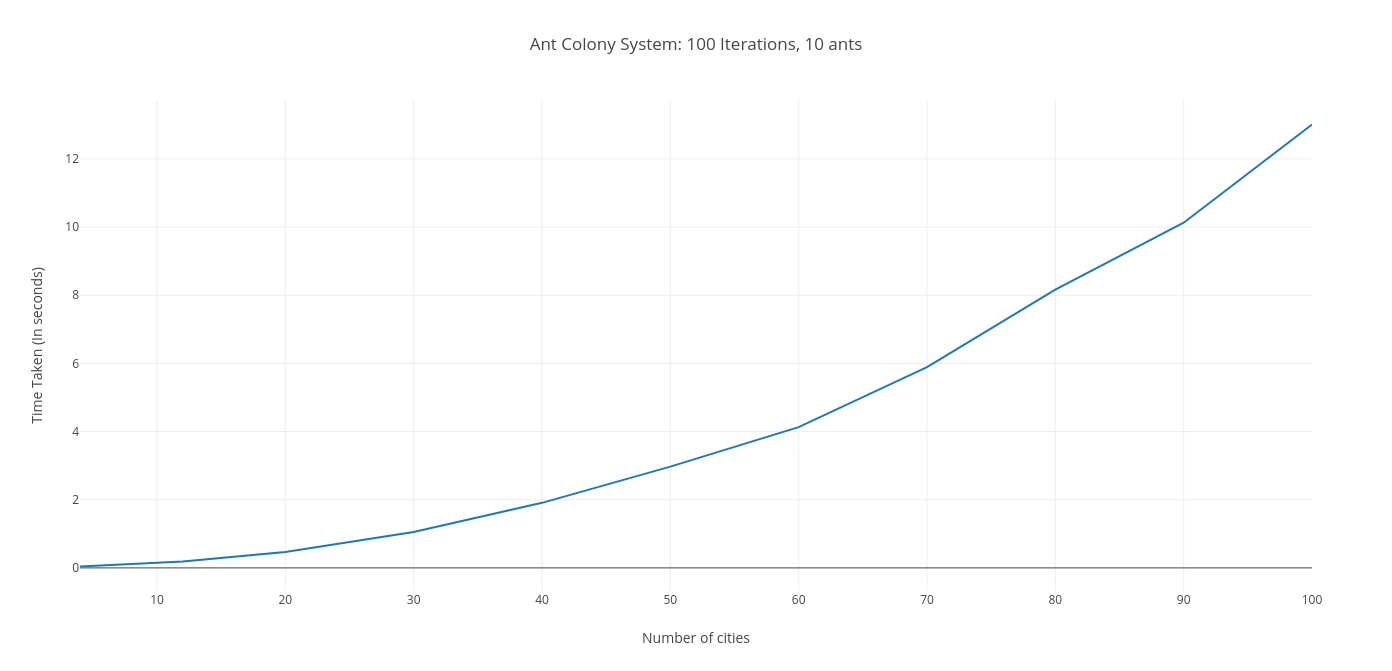
\includegraphics[scale=0.2]{ant1.png} \end{center}
\noindent
This can be improved using further optimisation methods \emph{e.g} nearest neighbour search and 3-OPT methods. These optimizations are suitable for TSPs of large sizes. 

\subsection{Complexity Analysis of Ant Colony System}
Complexity of ant colony system (ACS) method is quite high, especially for problems with hundereds of cities. The reason being essentially two loops in every pheromone update. And so the complexity is $\Omega(n^2)$. Computational Complexity of Ant Colony has been studied by Sudholt et. al. (2012) \cite{Sudholt2012}. One idea of an improvment can be selecting a certain number of neighbouring cities which are yet to be visited in every transition, and thus reducing the time complexity as not all cities have to be searched in every update. \cite{neumann2009computational}. Other optimization methods such as MAX-MIN Ant System provide for a faster implementation of ant colony optimization. In MMAS, maximum and minimum pheromone amounts ($\tau_max$, $\tau_min$) are added. Only global best or iteration best tour deposited pheromones. All edges are initialized to $\tau_min$ and reinitialized to $\tau_max$ when nearing stagnation.\cite{Sttzle1998}

\section{Genetic Algorithm}
\subsection{Introduction}
We present in this report the main description for the attached source code to solve Travelling salesman Problem. \newline \newline
As illustrated in the figure below, the main algorithm pipeline contains several main components:
\begin{enumerate}
    \item Initializing Algorithm Parameters
    \item Generate Initial Population
    \item Fitness Evaluation
    \item Parents Selection
    \item Crossover
    \item Mutation
    \item Generate New Population
\end{enumerate}
The following sections will explain briefly each components.
\newline \newline
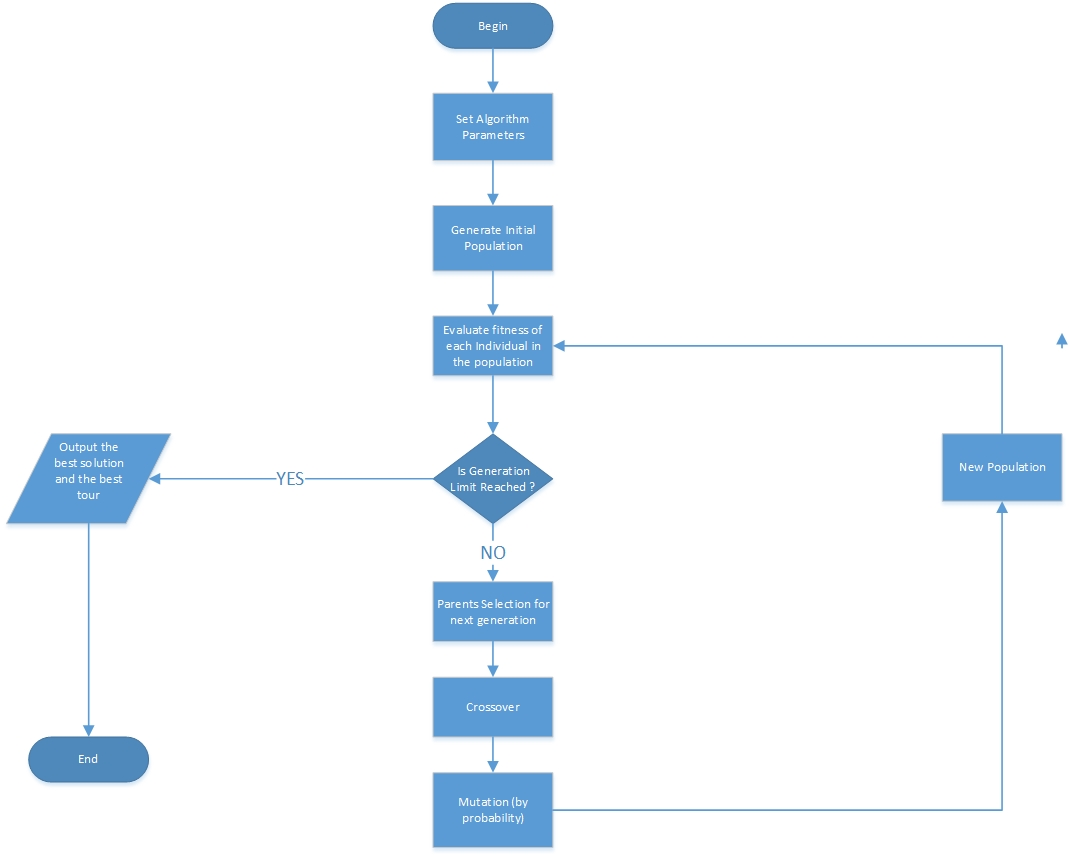
\includegraphics[width=\textwidth]{tsp-genetic-flowchart.jpg}

\subsection{Initializing Algorithm Parameters:}
In this step, several parameters should be initialized by the user. Specifically, \begin{enumerate}
    \item Max Population Size: 
    to specify the maximum number of individuals in any population
    \item Max Generation Numbers: usually the termination condition
    \item Mutation Rate: a real number in [0,1] specify the likelihood of mutation to happen
\end{enumerate}

\subsection{Generate Initial Population:}
In this step an initial generation is created randomly by creating a first random individual (Tour), and use shuffling on this individual until we reach the max population size. 
\subsection{Fitness Evaluation for Elitism:}
in this step, the fitness function for each individual should be calculated. For the TSP problem. the fitness function could be define as the total sum of distances for each tour.
This fitness function is used to evaluate how good each individual (Solution). Consequently, the fittest individual is elited to the next generation directly.
\subsection{Parents Selection:}
In this step, parents are chosen to mate together (crossover) and have a new individual. the selection process could be done in several ways. we applied Roulette Selection (with flexibility in the code to add new other selection algorithms without changing the code).
the basic of Roulette Selection is to pick a parent randomly according to weighted probability for each individual. the weights here represented by the fitness of the individual. In other words, individuals with high fitness function, have higher probabilities to be selected.
\subsection{Crossover:}
The crossover is the process of merging two individuals to have a new ones. there is several ways to implement the crossover. in our case, we implemented the Single Point Crossover. where a random point is generated bounded by the length of the solution. Afterwards, a new individuals are generated by taking the first part (before the picked point) from the first parent and the rest from the other taking into account the satisfaction of TSP constraints (no duplication) 
\subsection{Mutation:}
Each individual might undergo a mutation with a probability (specified in the parameters). the mutation basically is done by scanning the individual genes and picking a random number (bounded by the length of tour) and swap the current gene with the randomly picked one.
\subsection{Generate New Population:}
We keep repeating steps 5,6,7 until we have a full new population (enhanced one). and we go back to step 4 while we have not reached the generation limit.

\subsection{Complexity}

\begin{center}
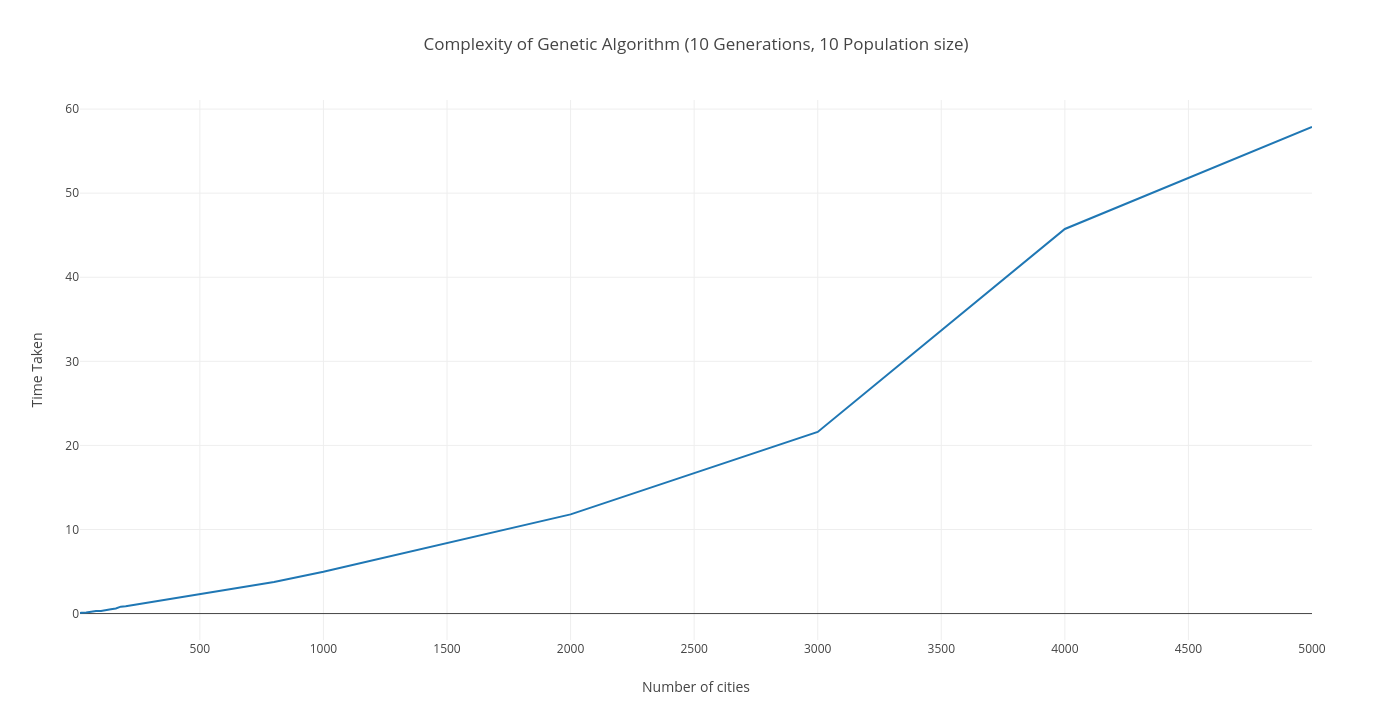
\includegraphics[scale=0.25]{genetic1.png}
\end{center}

\begin{center}
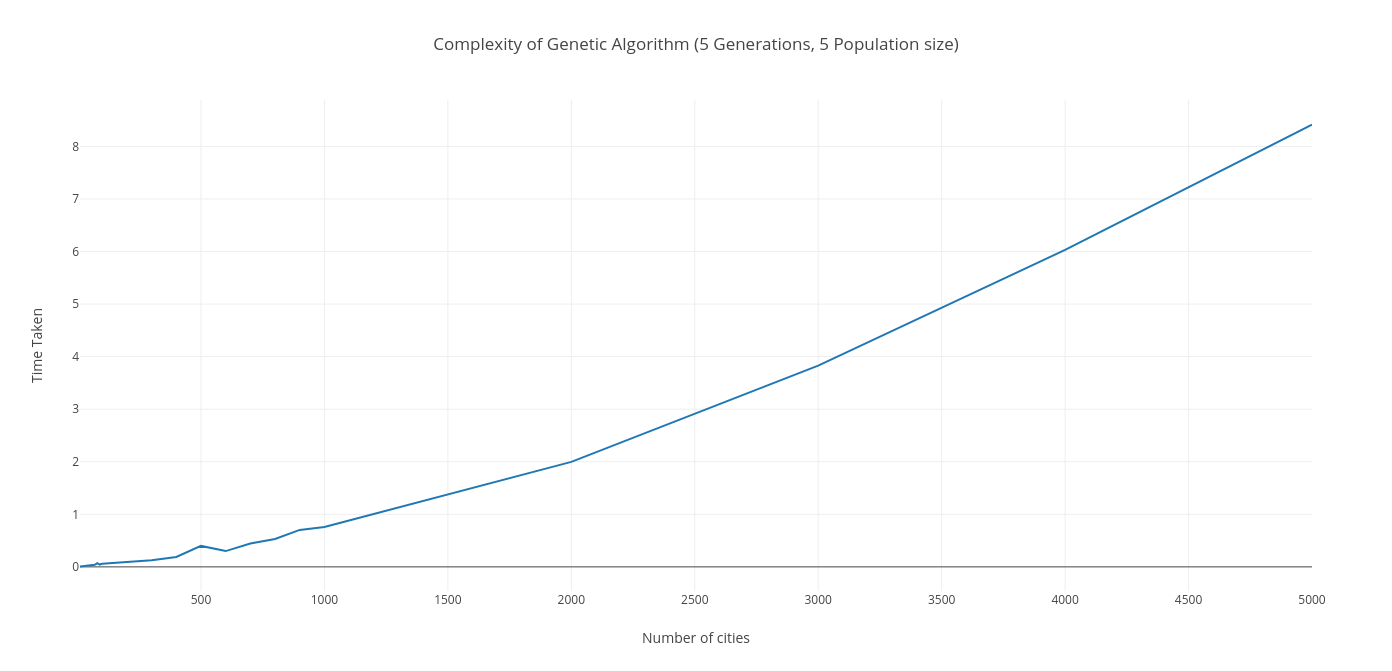
\includegraphics[scale=0.25]{genetic2.png}
\end{center}

\begin{center}
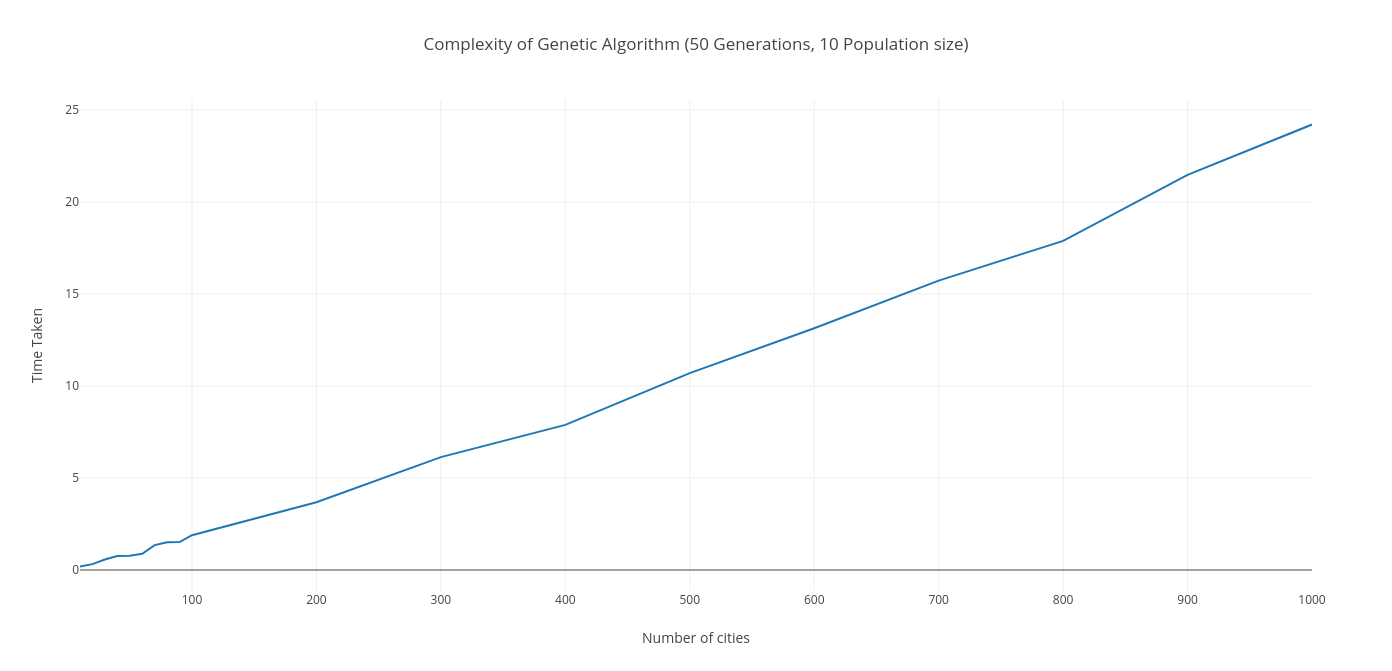
\includegraphics[scale=0.25]{genetic3.png}
\end{center}

\section{Greedy Algorithm}
	The greedy algorithm proceeds by applying a local optimal choice at each node. This strategy can sometimes provide a global optimal but it's not always the case. In most cases it provides an approximation of the optimal solution to the problem.
	
\subsection{Details of implementation}

	\begin{center}
	\colorbox[gray]{0.95}{
	\begin{minipage}{0.65\textwidth}
	\begin{algorithm}[H]
		\KwData{m x m Adjacency matrix}
		\KwResult{Tour of length (m+1) and total cost of the tour }
		\bigskip
		$\textit{tour}$ $\leftarrow$ [0] \\
		$\textit{totatl\_cost}$ $\leftarrow$ 0 \\
		
		\While{not all nodes visited}{
			$\textit{current\_node}$ $\leftarrow$ last element in $\textit{tour}$\\
			
			$\textit{next\_node}$ $\leftarrow$ node with min weight (list of adjacent nodes)
			
			append $\textit{next\_node}$ to the end of $\textit{tour}$\\
			
			$\textit{total\_cost}$ += distance($\textit{current\_node}$, $\textit{next\_node}$)
		}
	
		append 0 to the end of $\textit{tour}$\\
		
		$\textit{total\_cost}$ += distance( $\textit{next\_node}$,  \textit{first\_node})
		
		return $\textit{tour}$ , $\textit{total\_cost}$\\
		\bigskip
		\caption{Greedy algorithm for the TSP}
	\end{algorithm}
	\end{minipage}}
	\end{center}

\subsection{Results}
\begin{table}[!h]
	The algorithm was run on the complete set of TSP-LIB problems (both symmetric and asymmetric). Following is a sample of these results to showcase strong and weak points of this algorithm.
	\bigskip
	
	\centering
	\begin{tabular}{|c|c|c|c|c|c|}
		\hline
		Problem Name & No of vertexes  & Execution Time(s) & Min Path Cost &  Library  \\
		\hline\hline
		att48.tsp & 48 & 12861 & $<$1 ms & Symmetric TSP\\
		\hline
		a280.tsp & 280 & 3213 & 8.808 ms & Symmetric TSP\\
		\hline
		fl1577.tsp & 1577 & 29178 & 328.72 ms & Symmetric TSP\\
		\hline
		fnl4461.tsp & 4461 & 223855 & 3525.013 ms & Symmetric TSP\\
		\hline
		rl11849.tsp & 11849 & 1118490 & 52218.616 ms & Symmetric TSP\\
		\hline\hline
		ftv33.atsp & 34 & 1683 & $<$1 ms & Asymmetric TSP\\
		\hline
		ftv170.atsp & 171 & 3923 & 6.13 ms & Asymmetric TSP\\
		\hline
		rbg443.atsp & 443 & 6183 & 42.4 ms & Asymmetric TSP\\
		\hline
		\hline
	\end{tabular}
	\begin{tablenotes}
		\small
		\item A set of .csv files are included in our github repository with the full set of results.
	\end{tablenotes}
	\caption{Summary of greedy results on the TSP-LIB}
	\label{greedy_table}
\end{table}

\subsection{Discussion}
From the implementation of the algorithm we can see it has a complexity of $O(n)$. This makes the algorithm efficient in approximating even the biggest problem in a very reasonable time. And this can be seen in the results section, as even the \textit{rl11849.tsp} problem with 11849 vertexes took less than a minute to run.\\
However, the weak side of this algorithm is that it provides only an approximation rather than the optimal solution. This makes it suitable for problem with large \textit{n} values, where the optimal solution is not necessarily required and an approximation would be enough.



\section{MST Algorithm}
The Minimum Spanning Tree (MST) approach in the TSP problem starts by generating an MST for the problem's graph (which is defined by a tree that connects all the vertexes in a graph with the least possible overall weight of edges). Then a Depth First Search (DFS) is applied to acquire the tour path for the TSP.

\subsection{Details of implementation}

\begin{center}
	\colorbox[gray]{0.95}{
		\begin{minipage}{0.75\textwidth}
			\begin{algorithm}[H]
				\KwData{m x m Adjacency matrix}
				\KwResult{Tour of length (m+1) and total cost of the tour }
				\bigskip
				$\textit{T}$ $\leftarrow$ $\phi$ \\
				$\textit{U}$ $\leftarrow$ [0] \\
				
				\While{U $\neq$ V}{
					let (u, v) be the lowest cost edge such that u $\in$ U\ and$\>$ v $\in$ V - U
					
					T = T $\cup$$\>$ \{(u, v)\}
					
					U = U $\cup$$\>$ \{v\}\\
				}
			
				tour = DFS (T, u)
				
				
				return $\textit{tour}$ , $\textit{total\_cost}$\\
				\bigskip
				\caption{MST algorithm for the TSP}
			\end{algorithm}
	\end{minipage}}
\end{center}

\subsection{Results}
\begin{table}[!h]
	The algorithm was run on the complete set of TSP-LIB problems (both symmetric and asymmetric). Following is a sample of these results to showcase strong and weak points of this algorithm.
	\bigskip
	
	\centering
	\begin{tabular}{|c|c|c|c|c|c|}
		\hline
		Problem Name & No of vertexes  & Execution Time(s) & Min Path Cost &  Library  \\
		\hline\hline
		att48.tsp & 48 & 13926 & $<$1 ms & Symmetric TSP\\
		\hline
		a280.tsp & 280 & 3436 & 26.90 ms & Symmetric TSP\\
		\hline
		fl1577.tsp & 1577 & 29411 & 1012.26 ms & Symmetric TSP\\
		\hline
		fnl4461.tsp & 4461 & 248612 & 7920.18 ms & Symmetric TSP\\
		\hline
		rl11849.tsp & 11849 & 1384790 & 76464.248 ms & Symmetric TSP\\
		\hline\hline
		ftv33.atsp & 34 & 1712 & 1.02 ms & Asymmetric TSP\\
		\hline
		ftv170.atsp & 171 & 5032 & 9.95 ms & Asymmetric TSP\\
		\hline
		rbg443.atsp & 443 & 7561 & 73.76 ms & Asymmetric TSP\\
		\hline
		\hline
	\end{tabular}
	\begin{tablenotes}
		\small
		\item A set of .csv files are included in our github repository with the full set of results.
	\end{tablenotes}
	\caption{Summary of greedy results on the TSP-LIB}
	\label{greedy_table}
\end{table}

\subsection{Discussion}
The MST algorithm consists of two main parts; creating the minimum spanning tree and then searching the tree in a depth first manner, by analyzing the implementation: extracting the edge with the lowest cost is $O(log(V))$. This means creating the MST's complexity is $O(Vlog(V))$. That makes the total complexity for the algorithm $O(Vlog(V) + V)$.\\
As for the strong and weak points of the algorithm we can draw a lot of similarities to the greedy algorithm. It's very efficient in approximating huge problems as shown in the results table. But also it only approximates a solution and doesn't usually provide an optimal one.

\bibliographystyle{ieeetr}

\bibliography{TSP_Report}

\end{document}  
